In our system there are four main layers, which are classified as web interface layer, wireless connection layer, base station layer, camera layer. The user can communicate with the remote surveillance camera with the help of the user interface. The Ethernet and black box will bridge between the user and the remote camera. User interface will include all kinds of resources that user is capable of using. In the system streaming video is made available and some of the controls that user can use through his computer. In the camera layer we have our camera module, which can be rotated and tilted 180 degrees, which makes it 360- degree total movement possible. In the network layer we will be using Ethernet connection. The source of the power for the camera layer and black box is base station. The main power source for the base station is solar battery.



\begin{figure}[h!]
	\centering
 	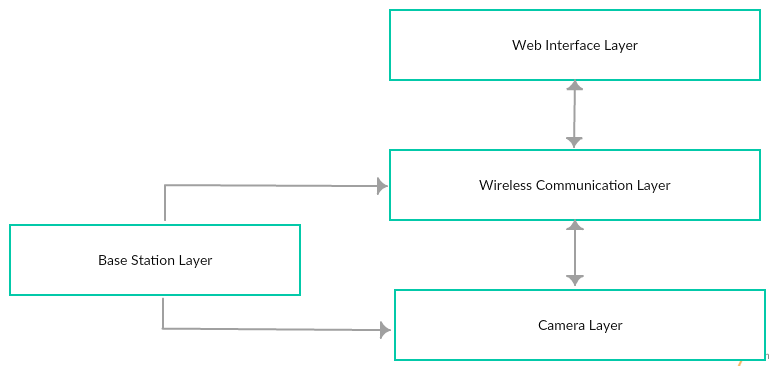
\includegraphics[width=0.90\textwidth]{architectural design specification latex/images/ADS diagrams/layers.png}
 \caption{System architecture}
\end{figure}
